\documentclass[10pt,portrait, twocolumn]{article}
\usepackage{multicol}
\usepackage{calc}
\usepackage[portrait]{geometry}
\usepackage{amsmath,amsthm,amsfonts,amssymb}
\usepackage{times}
\usepackage{color,graphicx,overpic}
\graphicspath{ {images/} }
\usepackage{hyperref}
\usepackage{pgfplots}
\usepackage{esint}
\usepackage{bm}
\usepackage{tikz}
\usepackage{relsize}
\usepackage{datetime}
\usepackage{circuitikz}
\usepackage[utf8] {inputenc}
\usepackage[spanish, activeacute] {babel}
\usepackage{IEEEtrantools}
\usetikzlibrary{arrows}

\usepackage{framed}

\usepackage{pdflscape}

%Evita errores con el paquete de español y escribir flechas entre tikz nodos
\tikzset{
every picture/.append style={
  execute at begin picture={\deactivatequoting},
  execute at end picture={\activatequoting}
  }
}

\usepackage{draftwatermark}
\SetWatermarkText{Javier de Martín}
\SetWatermarkScale{0.8}

% This sets page margins to .5 inch if using letter paper, and to 1cm
% if using A4 paper. (This probably isn't strictly necessary.)
% If using another size paper, use default 1cm margins.
\geometry{top=.5cm,left=.5cm,right=.5cm,bottom=.5cm}
    
\pgfplotsset{
    dirac/.style={
        mark=triangle*,
        mark options={scale=2},
        ycomb,
        scatter,
        visualization depends on={y/abs(y)-1 \as \sign},
        scatter/@pre marker code/.code={\scope[rotate=90*\sign,yshift=-2pt]}
    }
}

% Turn off header and footer
\pagestyle{empty}

% Redefine section commands to use less space
\makeatletter
\renewcommand{\section}{\@startsection{section}{1}{0mm}%
                                {-1ex plus -.5ex minus -.2ex}%
                                {0.5ex plus .2ex}%x
                                {\normalfont\large\bfseries}}
\renewcommand{\subsection}{\@startsection{subsection}{2}{0mm}%
                                {-1explus -.5ex minus -.2ex}%
                                {0.5ex plus .2ex}%
                                {\normalfont\normalsize\bfseries}}
\renewcommand{\subsubsection}{\@startsection{subsubsection}{3}{0mm}%
                                {-1ex plus -.5ex minus -.2ex}%
                                {1ex plus .2ex}%
                                {\normalfont\small\bfseries}}
\makeatother

\newcommand{\Lagr}{\mathcal{L}}

% Define BibTeX command
\def\BibTeX{{\rm B\kern-.05em{\sc i\kern-.025em b}\kern-.08em
    T\kern-.1667em\lower.7ex\hbox{E}\kern-.125emX}}

% Don't print section numbers
\setcounter{secnumdepth}{0}


\setlength{\parindent}{0pt}
\setlength{\parskip}{0pt plus 0.5ex}

%My Environments
\newtheorem{example}[section]{Example}
% ---------------------------------------------------------------

\begin{document}

\begin{landscape}

\raggedright
\footnotesize
\begin{multicols}{3}


% multicol parameters
% These lengths are set only within the two main columns
%\setlength{\columnseprule}{0.25pt}
\setlength{\premulticols}{1pt}
\setlength{\postmulticols}{1pt}
\setlength{\multicolsep}{1pt}
\setlength{\columnsep}{2pt}

\begin{framed}
	\begin{center}
    	\Large{\underline{Sistemas de Radiocomunicación}} \\
    	\scriptsize{3º Ingeniería de Telecomunicaciones | UPV/EHU}\\
     	%Actualizado por última vez el \today \\
     	"\textsl{Under-promise and over-deliver}." \\
     	%\hspace{5 pt} \\
     	\small{\textbf{Javier de Martín -- 2017}}
	\end{center}
\end{framed}

\section{\underline{2. }}

\subsection{Antena Transmisora}

\begin{circuitikz}[scale=.8, transform shape, european]

	\draw[fill] (-.15,0) circle[radius = 1pt];
	\draw[fill] (-.15,-2) circle[radius = 1pt] node[below]{g};
	\draw[fill] (5, -2) node[below]{d};
	
	\draw (-3,0) 
		to[sV, l_= $V_{TX}$] (-3,-2)
		(-3,0) to[R  = $Z_{O}$] (0,0);
	\draw (0,0) 
		to[R  = $R_{\Omega}$] (2,0)
		to[R  = $jX_{in}$] (4,0)
		-- (5,0)
		to[R  = $R_{r}$] (5,-2)
		-- (-3,-2);
		
	\draw[-latex] (-.3,-1.9) -- (-.3,-.1) node[midway, left] {$P_{in}^{'}$};
	\draw[-latex] (0,-1.9) -- (0,-.1) node[midway, right] {$P_{in}$};
	
	\draw (-1.5, -.5) node[]{(1)};
	\draw (2.5, -.5) node[left]{(2)};
\end{circuitikz}

(1) Pérdidas por desadaptación y (2) pérdidas óhmicas

\begin{equation*}
Z_{in} = R_{R} + R_{\Omega} + j \cdot X_{in}
\end{equation*}

\begin{equation*}
P_{in} = P_{in}' \cdot ( 1 - |\rho|^{2})
\end{equation*}

\begin{equation*}
P_{r} = \eta \cdot P_{in} = I^{2} \cdot R_{r}
\end{equation*}

\begin{equation*}
\rho = \frac{Z_{in} - Z_{o}}{Z_{in} + Z_{o}} \hspace{10pt} \eta = \frac{R_{R}}{R_{R} + R_{\Omega}}
\end{equation*}

\begin{equation*}
G \cdot P_{in} = D \cdot P_{r} \hspace{10pt} G = D \cdot \eta
\end{equation*}

\subsection{Antena Receptora}

     \begin{circuitikz}[scale=.8, transform shape, european]

	\draw[fill] (4,0) circle[radius = 1pt];
	\draw[fill] (4,-2) circle[radius = 1pt] node[below]{$g_{RX}$};
	\draw[fill] (-2, -2) circle[radius = 1pt] node[below]{$d_{RX}$};
	
	\draw (-3,0) 
		to[sV, l_= $V_{TX}$] (-3,-2)
		(-3.5,-1) node[right]{$P_{RX}$}
		(-3,0) to[R  = $R_{r}$] (0,0);
	\draw (0,0) 
		to[R  = $R_{\Omega}$] (2,0)
		to[R  = $jX_{in}$] (4,0)
		-- (5.5,0)
		to[R  = $R_{RX}$] (5.5,-2)
		-- (-3,-2);
		
	\draw[-latex] (3.9,-1.9) -- (3.9,-.1) node[midway, left] {$P_{RX}^{'}$};
	\draw[-latex] (3.9,-1.9) -- (3.9,-.1) node[midway, right] {$P_{RX}$};
	\draw[-latex] (0,-1.9) -- (0,-.1) node[midway, left] {$P_{L}$};
	
	\draw[dashed] node[draw,minimum width=2cm,minimum height=2.4cm,anchor=south west] at (4.9,-2.2){}
		(6,-2.4) node[]{Bloque Receptor};
		
	\draw (-.4, -.5) node[]{(1)};
	\draw (6.5, -.5) node[left]{(2)};
\end{circuitikz}

(2) Pérdidas por desadaptación y (1) pérdidas óhmicas


\begin{equation*}
A_{ef} = \frac{\lambda^{2}}{4 \pi} \cdot D_{RX}
\end{equation*}

?`Qué potencia llega a $R_{RX}$?

Pérdidas óhmicas:

	\begin{equation*}
	P_{RX}`= P_{L} \eta_{l} \cdot R_{RX} \rightarrow  \eta_{l} R_{X} = \frac{R_{R}}{R_{R} + R_{\Omega}}
	\end{equation*}
	
Pérdidas por desadaptación:

	\begin{equation*}
	P_{RX} = P_{RX}' (1 - |\rho_{RX}|^{2}) \rightarrow P_{RX} = \frac{Z_{RX} - Z_{ANT_{RX}}}{Z_{RX} + Z_{ANT_{RX}}}
	\end{equation*}


\begin{IEEEeqnarray*}{rCl}
			P_{L} & = & \frac{P_{R} \cdot D_{TX}}{4 \pi r^{2}} \cdot \frac{\lambda^{2}}{4 \pi} \cdot D_{RX} \\
				 & = & P_{R} \cdot D_{TX} \left( \frac{\lambda}{4 \pi r} \right)^{2} D_{RX}
		\end{IEEEeqnarray*}


Fórmula de Friis:

	\begin{equation*}
	P_{r} - D - L_{FS} + D_{RX} = P_{L}
	\end{equation*}

\end{multicols}

\end{landscape}



\begin{framed}
	\begin{center}
    	\Large{\underline{Sistemas de Radiocomunicación}} \\
	\large{Primera Parte} \\
    	\scriptsize{3º Ingeniería de Telecomunicaciones | UPV/EHU}\\
     	%Actualizado por última vez el \today \\
     	"\textsl{Under-promise and over-deliver}." \\
     	%\hspace{5 pt} \\
     	\small{\textbf{Javier de Martín -- 2017}}
	\end{center}
\end{framed}

%%%%%%%%%%%%%%%%%%%%%%%%%%%%%%%%%%%
%% TEMA 1 - INGENIERIA DEL ESPECTRO RADIOELECTRICO %%
%%%%%%%%%%%%%%%%%%%%%%%%%%%%%%%%%%%

\section{\underline{1. Ingeniería del Espectro Radioeléctrico}}

\textbf{?`Qué es la radiocomunicación?} \textbf{Radiocomunicación} Telecomunicación basada en ondas de radio. \textbf{Telecomunicación}: Cualquier transmisión o recepción de información por aire, radio, cable o cualquier otro sistema de electromagnetismo. \textbf{Radio}: Término general aplicado al uso de ondas de radio. \textbf{Ondas de Radio}: Ondas EM con frecuencias arbitrariamente menores a 3000 GHz (excepto la luz), que se propaga en el espacio sin necesidad de guías artificiales.

El espectro de radio varía desde los 3kHz hasta los 300GHz y es una parte pequeña del espectro electromagnético.\\

\scalebox{.7}{\begin{tabular}{|c|c|c|c|c|c|c|}\hline VLF & LF & MF & VHF & UHF & SHF & EHF \\\hline 3-30 kHZ & 30-300 kHZ & 300kHz - 3MHz & 3-30MHz & 30-300MHz & 3-30GHz & 30-300GHz \\\hline \end{tabular}}\\

Bandas de frecuencia según EBU (European Broadcasting Union)

	\begin{center}
\begin{tabular}{|l|l|}
\hline
Banda I   & 41-68MHz    \\ \hline
Banda II  & 87,5-108MHz \\ \hline
Banda III & 162-230MHz  \\ \hline
Banda IV  & 470-582MHz  \\ \hline
Banda V   & 582-960MHz  \\ \hline
Banda VI  & 12 GHz      \\ \hline
\end{tabular}
	\end{center}
	
Bandas según ITU, nomenclatura de Radar

	\begin{center}
	\begin{tabular}{|l|l|}
\hline
L  & 1-2 GHz    \\ \hline
S  & 2-4 GHz    \\ \hline
C  & 4-8 GHz    \\ \hline
X  & 8-12 GHz   \\ \hline
Ku & 12-18 GHz  \\ \hline
K  & 18-27 GHz  \\ \hline
Ks & 27-40 GHz  \\ \hline
mm & 40-300 GHz \\ \hline
\end{tabular}
	\end{center}
	
El espectro de radiocomunicación es un recurso natural limitado pero reutilizable. La limitación es debida a las características de propagación de las ondas de radio, disponibilidad de la tecnología y equipamiento para diferentes aplicaciones y disponibilidad de bandas de frecuencias adecuadas para aplicaciones específicas. La demanda del espectro siempre ha sido mayor que su disponibilidad.\\

Sólo hay un único espectro de radio, es únicamente expandible hasta las ondas de longitud de onda milimétrica o empleando métodos de codificación. Las ondas de radio no respetan las fronteras internacionales, edificios u otros.

\subsection{Gestión del Espectro}

La \textbf{ITU} (International Telecommunication Union) atribuye el espectro global y órbitas de satélite, desarrollar estándares técnicos que aseguren la interconexión de redes y tecnologías y forzar la mejora del acceso a ICTs en comunidades subdesarrolladas.\\

Las \textbf{WRC} (World Radiocommunication Conferences) de la ITU se celebran cada tres años en Ginebra, revisan las regulaciones de radio, el uso del espectro y cualquier otro aspecto.\\

La \textbf{ETSI} (European Telecommunication Standards Institute) crea estándares para tecnologías de radio. Fundada inicialmente para cubrir las necesidades europeas ha crecido para ser respetada como un estándar mundial.

\begin{center}
\begin{tabular}{l|c|c|}
\cline{2-3}
                                            & \textbf{English} & \textbf{Spanish} \\ \hline
\multicolumn{1}{|l|}{\textbf{Servicios}}    & Allocation       & Atribución       \\ \hline
\multicolumn{1}{|l|}{\textbf{Áreas/Paises}} & Allotment        & Adjudicación     \\ \hline
\multicolumn{1}{|l|}{\textbf{Estaciones}}   & Assignment       & Asignación       \\ \hline
\end{tabular}
\end{center}

\begin{itemize}
	\item \textbf{Allocation} (of a frequency band): Entrada en la tabla de atribución de frecuencias de una banda de frecuencia dada para el propósito por uno o más servicios de radiocomunicación terrestres o espaciales. Este término también se aplica a la banda de frecuencias afectada.
	\item \textbf{Allotment} (of a radio frequency or radio frequency channel): Entrada de un canal de frecuencias en un plan acordado, es adoptado por una conferencia competente, para usarlo en uno o más administraciones para radiocomunicación terrestre o espacial un uno o más países o áreas geográficas bajo unas condiciones especificadas.
	\item \textbf{Assignment} (of a radio frequency or a radio frequency channel): Autorización proporcionada por una administración para que una estación de radio pueda utilizar una frecuencia o un canal de radiofrecuencia bajo unas condiciones especificadas.
\end{itemize}

\begin{figure}[h]
	\centering
     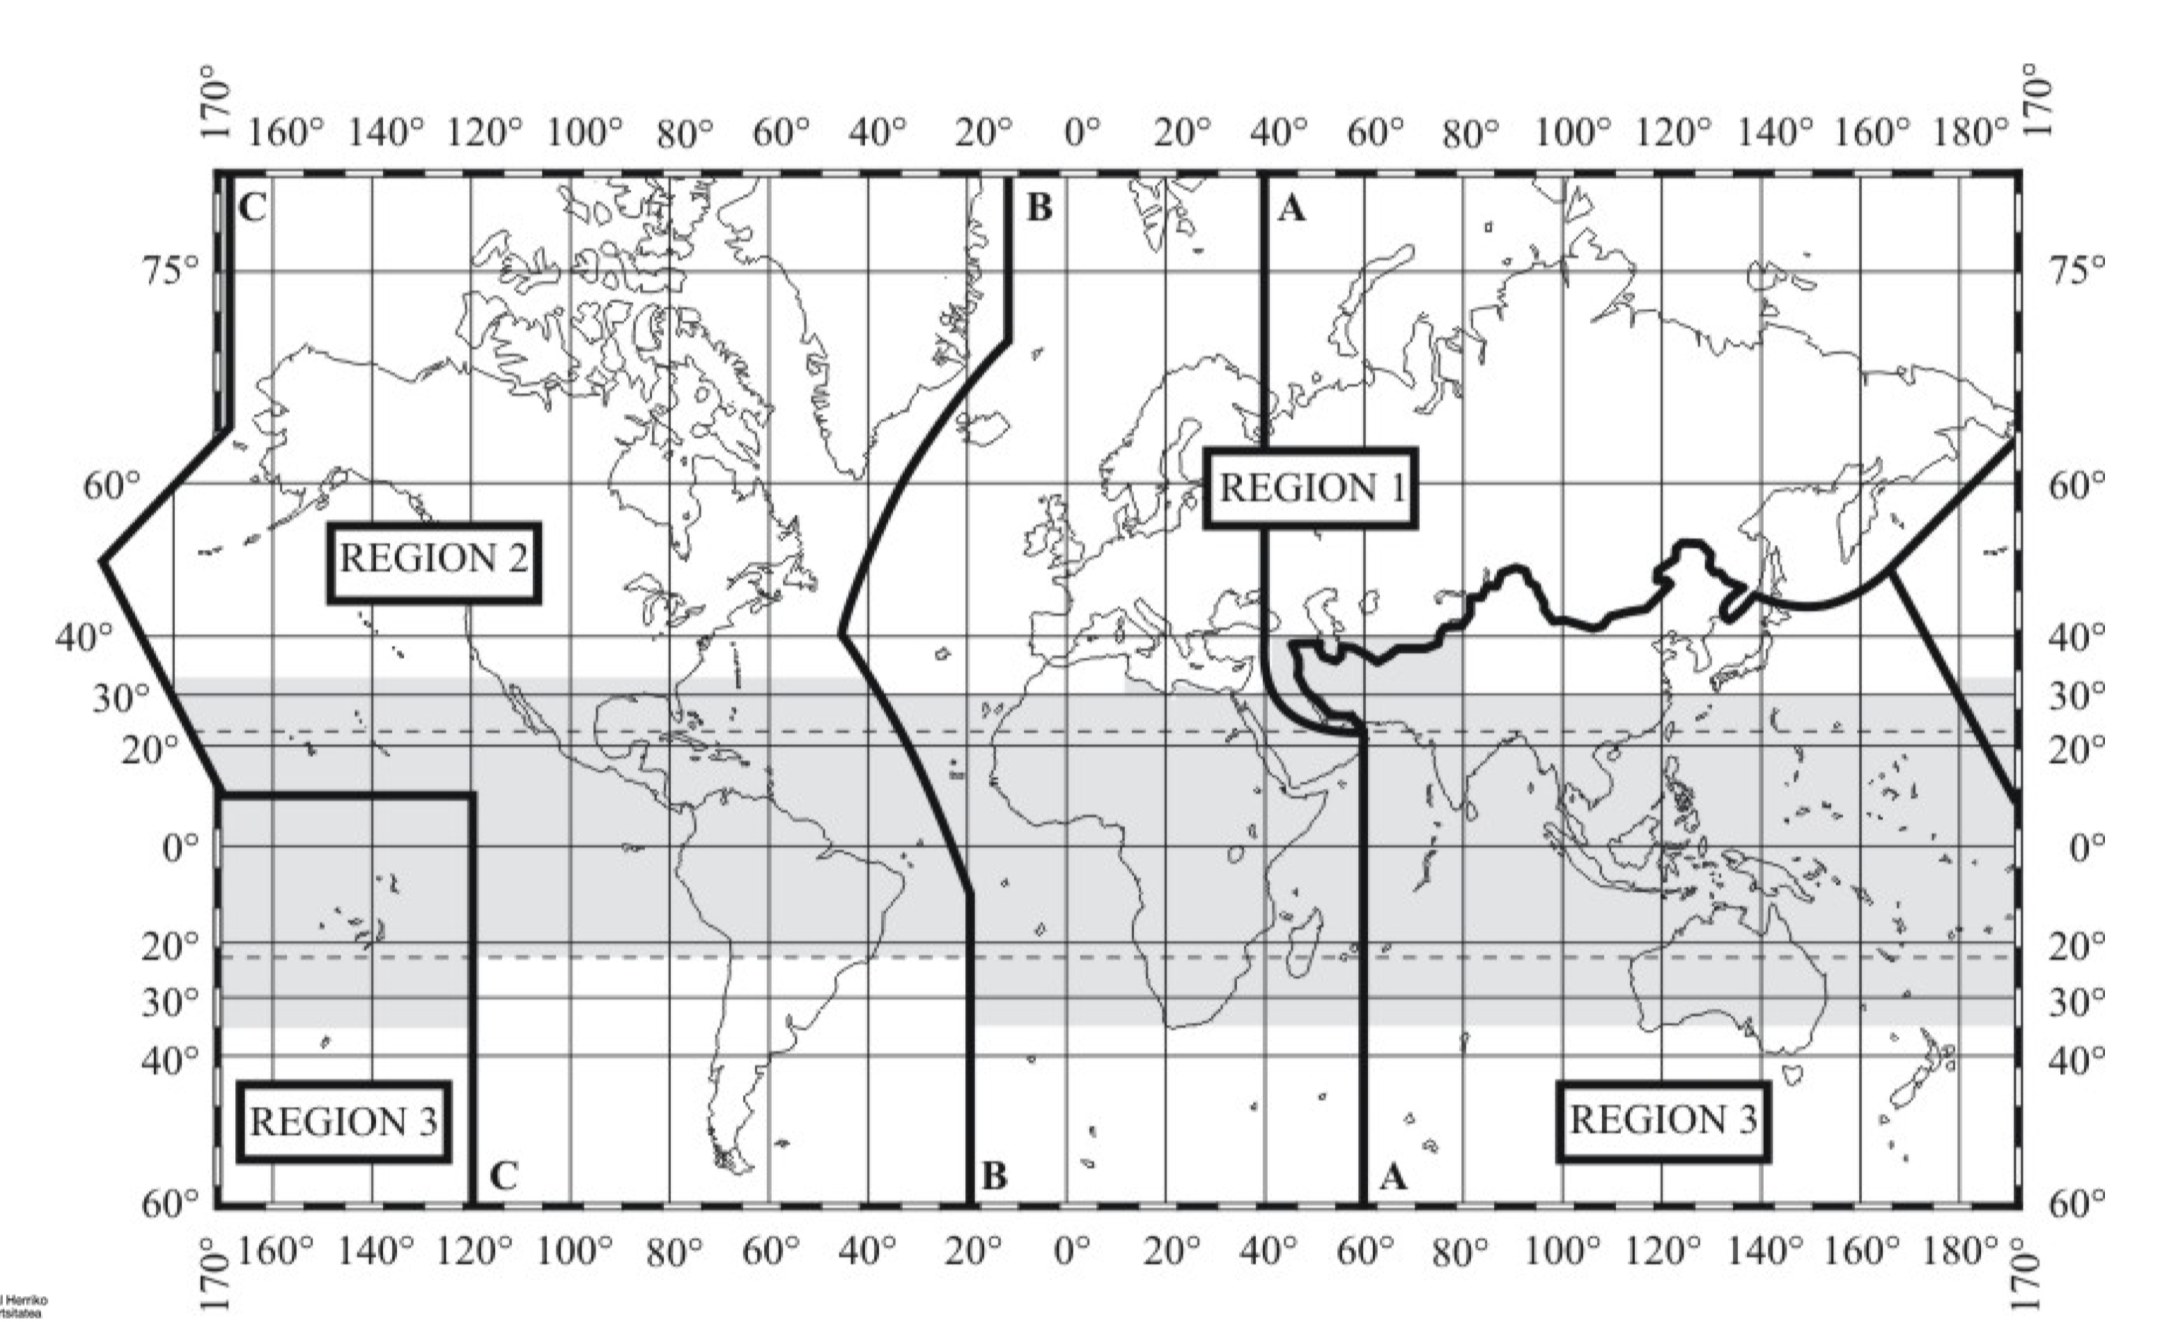
\includegraphics[width=0.5\textwidth]{Regiones}
      \caption{Regiones de frecuencias}
\end{figure}

Hay varios \textbf{tipos} de atribuciones de frecuencias:

	\begin{itemize}
		\item \textbf{Exclusiva}: Atribución para un servicio de radio.
		\item \textbf{Compartido}: Atribución para varios servicios de radio.
	\end{itemize}
	
\textbf{Categorías} de servicios:

	\begin{itemize}
		\item \textbf{Primarios}: Prioridad en la elección de las frecuencias, escrito en mayúsculas.
		\item \textbf{Secundario}: No pueden producir interferencias a estaciones primarias. No pueden reclamar protección por interferencia a estaciones de servicios primarios. Pueden reclamar protección contra interferencias de estaciones del mismo servicio u otros servicios secundarios.
	\end{itemize}
	
La \textbf{gestión del espectro} refleja muchas actividades: Planificación del uso del espectro, atribución y asignación de licencias del espectro, interacción con organizadores regionales e internacionales... Históricamente, los reguladores han asignado las frecuencias emitiendo licencias a usuarios específicos para usos específicos $\rightarrow$ Método Administrativo. Hay formas más flexibles de licencia, las bandas se pusieron a disposición de varios usos en vez de sólo para uno y se introdujeron subastas para asignar los espectros a los usuarios.\\

El \textbf{modelo administrativo} es el utilizado por la mayoría de reguladores en el mundo. Los reguladores son las autoridades centrales para la asignación del espectro y decisiones de uso. Las decisiones de asignación son a menudo estáticas en dimensiones temporales y espaciales, es decir, son válidas para períodos de tiempo muy largos y para grandes regiones geográficas por lo que no resulta muy eficiente.\\

El \textbf{modelo de mercado} dice que los recursos del espectro de radiocomunicación debería ser tratado como propiedad privada. La asignación debe de er implementada por las fuerzas de mercado. Los propietarios del espectro deberían ser capaces de comerciar esas partes en mercados secundarios. Los propietarios de espectro podrán utilizar su banda de la manera que quieran a través de cualquier tecnología.\\

La \textbf{teoría del espectro libre} proporciona acceso libre a cualquier espectro para cualquier uso, está necesitada de regulaciones para poner orden.\\

A vistas de \textbf{futuro} se preveé una mayor demanda del espectro disponible, planes centrados en incrementar la compartición del espectro entre servicios, planes centrados en la liberación del espectro no utilizado o no utilizado eficientemente.\\

Las \textbf{licencias} se asignan a estaciones de radio para usuarios específicos con usos específicos y asignadas en subastas. El espectro \textbf{sin licencia} tiene frecuencias para aplicaciones ISM y SDR, limitando la potencia emitida, cualquiera puede transmitir sin una licencia mientras cumpla con las reglas para limitar/evitar interferencias, las principales bandas sin licencias fueron aquellas diseñadas como industriales, científicas y médicas (ISM). En los últimos 15 años ha crecido la demanda en el uso del espectro sin licencia.

\hrulefill

\section{\underline{2. Tecnologías Básicas de Radio}}

\subsection{Bloques de un sistema de radiocomunicación genérico}

\begin{figure}[h]
	\centering
     \begin{tikzpicture}
 	\node at (0,0) [circle,draw] (Antena1) {Antena};
        \node at (3,0) [rectangle,draw] (Medio) {Medio};
        \node at (6,0) [circle, draw] (Antena2) {Antena};
        \node at (0,-2) [rectangle, draw] (Transmisor){Transmisor};
        \node at (3,-2) [rectangle,draw] (Perturbaciones){Perturbaciones};
        \node at (6,-2) [rectangle, draw] (Receptor){Receptor};
        \node at (0,-4) [circle,draw](Fuente)  {Fuente};
        \node at (6,-4) [circle,draw](Display) {InfoDisplay};
        
        
        \draw[->, blue, thick] (Fuente) -- (Transmisor);
        \draw[->, blue, thick] (Transmisor) -- (Antena1);
        \draw[->, red, thick] (Antena1) -- (Medio);
        \draw[->, red, thick] (Medio) -- (Antena2);
        \draw[->, blue, thick] (Receptor) -- (Display);
        \draw[->, blue, thick] (Perturbaciones) -- (Receptor);
        \draw[->, blue, thick] (Perturbaciones) -- (Transmisor);
        \draw[->, blue, thick] (Perturbaciones) -- (Medio);
        \draw[->, blue, thick] (Antena2) -- (Receptor);
        
	\node at (3,-4) [blue] {Señal};
	\node at (3,-4.3) [red]{Radiación};

	\end{tikzpicture}
      \caption{Esquema general}
  \end{figure}

\begin{center}
\subsection{Codificación, Entrelazado y Modulación}
\end{center}

\textbf{Codificación}: En cualquier comunicación digital surgen errores cuando algunos de los bits son recibidos con el valor incorrecto. En los sistemas de radiocomunicación los errores son frecuentes debido a la baja potencia de la señal recibida $C$. La codificación de canal o FEC (Forward Error Correction) permiten detectar y corregir bits erróneos añadiendo bits redundantes a los bits de datos.

	\begin{equation*}
		\text{Code Rate} = \frac{\text{Bits de datos}}{\text{Bits totales}}
	\end{equation*}

\textbf{Entrelazado}:  Mezclar los bits en el codificador para reordenarlos en el receptor. Si los errores ocurren en ráfagas, los bits erróneos están menos uniformemente distribuidos al entrelazarlos. El inconveniente que tienen es el tiempo de latencia ya que el receptor tiene que esperar a que todos los bits lleguen para decodficarlos.\\

\textbf{Modulación}: Proceso de transferencia de información en banda base a la frecuencia del canal generada por el oscilador. Puede ser modulación en amplitud, fase o frecuencia. También puede ser una combinación de los parámetros anteriores.\\

\textbf{Filtrado del Canal}: Controlar el solape de los espectros adyacentes y reducir la interferencia entre símbolos (ISI), producida por la limitación del ancho de banda. Esto se consigue haciendo que la función de transferencia del filtro del canal es lo más cercana posible a la respuesta en frecuencia de Nyquist. Por el teorema de Nyquist se requiere, teóricamente, un mínimo de ancho de banda para detectar $R$ símbolos/s, sin ISI, es R/s Hz. Esto ocurre cuando la función de transferencia del sistema es rectangular y constante entre 0 y $1/2 \cdot T$. El factor de roll-off representa el exceso de ancho de banda requerido sobre el ancho ideal de Nyquist, siendo $\alpha = 0$ el ancho de banda ideal correspondiente al de Nyquist. Con $\alpha = 1$ se requiere el doble de ancho de banda.

	\begin{equation*}
	1 + \alpha \leq \text{BW}
	\end{equation*}
	
	\begin{figure}[h]
	\centering
       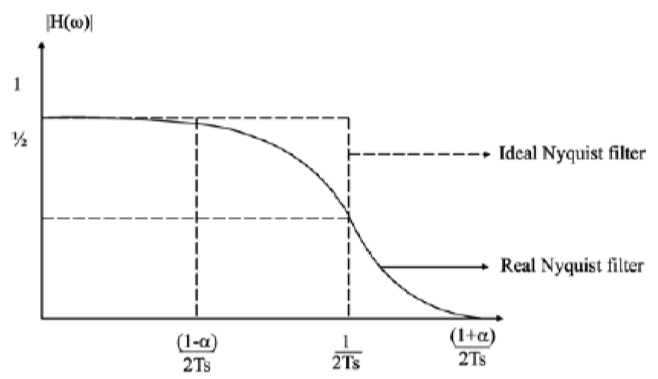
\includegraphics[width=0.35\textwidth]{Nyquist}
      \caption{Regiones de frecuencias}
\end{figure}

En una modulación binaria, cada bit corresponde a un nivel de modulación o símbolo. La tasa de modulación, $V_{s} (\text{símbolos} / \text{segundo}$), se expresa en baudios y coincide con el bitrate. La eficiencia espectral teórica de las modulaciones binarias es de $1 \text{bit}/\text{s}/\text{Hz}$.

	\begin{equation*}
	V_{s} (\text{baudios}) = V_{b} (\text{bit}/\text{s})
	\end{equation*} 
	
En las modulaciones multinivel, cada símbolo de $m$ bits se corresponde a un nivel de modulación. El número de estados o niveles de modulación es $M = 2^{m}$. Entonces, las relaciones entra tasas y períodos de símbolos ($V_{s}$ y $T_{s}$) y bits ($V_{b}$ y $T_{b}$) son:

	\begin{equation*}
	V_{s} (\text{baud}) = \frac{V_{b}}{log_{2}M} = \frac{V_{b}}{m} \hspace{20pt} T_{s} = \log_{2} M \cdot T_{b} = m \cdot T_{b}
	\end{equation*}
	
La eficiencia espectral teórica es:
	\begin{equation*}
	m = \log_{2}M \text{bits}/\text{s}/\text{Hz}
	\end{equation*}
	
Los \textbf{puntos de constelación} representan los estados de modulación. El módulo y fase del vector que une el origen con cada punto de la constelación, son la amplitud y fase de la portadora a ese nivel de modulación correspondiente al símbolo representado por ese punto.

\begin{figure}[h]
	\centering
       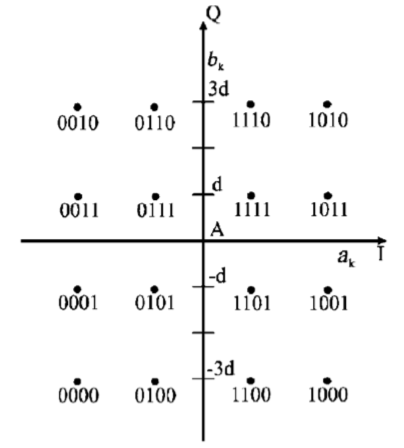
\includegraphics[width=0.2\textwidth]{IQ}
      \caption{Puntos de constelación}
\end{figure}

La distancia de decisión $d$ es la mitad de la distancia del segmento que une dos puntos consecutivos de la constelación. La asignación de los puntos se realiza mediante código Gray, los estados adyacentes de la constelación sólo difieren en un bit. El bit error rate disminuye cuando aparece error de demodulación.

\subsection{Transmisor}

Toma la señal IF modulada y la lleva al canal de RF y la amplifica para llegar al nivel de potencia requerido para ser transmitida. Normalmente se añade un filtro de canal RF en la etapa final para evitar radiar señales indeseadas. Los amplificadores de potencia son muy sensibles a la potencia reflejada por lo que es necesaria una adaptación de impedancias la antena transmisora. Hay sensores que miden la potencia reflejada y en el caso de la desadaptación de impedancias el transmisor de apaga para evitar daños. También los amplificadores de potencia son responsables de la degradación de la señal transmitida debido a la no linealidad. A la hora de diseñar transmisores hay que jugar con la eficiencia y la degradación de la señal.

\subsection{Antenas}

Son los elementos que adaptan las ondas guiadas, que son transmitidas por cable o guías a las ondas de radio que se propagan por el espacio, añadiendo características direccionales. Son las partes en los sistemas de telecomunicación encargadas de radiar o recibir las ondas electromagnéticas.\\
Normalmente las antenas son clasificadas de acorde a su geometría:

	\begin{itemize}
	\item \textbf{Antenas Lineales o de Cable}: Formadas por una varilla o cables. Los campos radiados se calculan por la corriente que circula por el cable.
	\item \textbf{Anenas de Apertura}: Formadas por una abertura en la cual se produce la radiación. Los campos radiados se calculan por los campos en la abertura. Dependiendo de cómo son generados los campos en la abertura se distinguen 5 antenas: bocinas, reflectoras, lentes, slots y patches.
	\item \textbf{Array de Antenas}: Formadas por un grupo de antenas operando como si fueran una única. Los patrones de radiación dependen principalmente en la disposición del array en lugar del diagrama de radiación de cada antena. Normalmente, las antenas son iguales pero en algunos casos pueden ser diferentes (Yagi o logperiódicas).
	\end{itemize}
	
Para analizar los \textbf{parámetros} que definen las características de una antena hay que tener en cuenta el \textbf{teorema de reciprocidad} que dice que las antenas tienen las mismas características estén transmitiendo o recibiendo.

	\begin{itemize}
		\item \textbf{Impedancia}: La antena será la última parte del sistema de transmisión y el amplificador de transmisión la verá como una carga. La antena es equivalente a una impedancia que disipa potencia generada en el generador. Esa potencia no es disipada sino radiada. Para maximizar la potencia transmitida, la impedancia del a antena y el transmisor de potencia deben estar adaptadas. La impedancia de entrada de la antena ($Z_{in}$, $Z_{a}$ o $Z_{en}$) es definida en los terminales de la antena como el cociente entre voltaje y corriente. En general, consiste en una parte real $R_{in}(f)$ y una parte imaginaria $X_{in}(f)$ $\rightarrow Z_{in}(f) = R_{in}(f) + j \cdot X_{in}(f)$. Si $Z_{in}(f)$ no tiene parte reactiva en alguna frecuencia en concreto ($X_{in} = 0$) se conoce a la antena como antena resonante para esa frecuencia.
		
			
			
			\begin{center}
\begin{circuitikz}[scale=.5, transform shape, european]

	\draw (0,0) 
		to[R  = $R_{\Omega}$] (2,0)
		to[R  = $jX_{in}$] (4,0)
		-- (5,0)
		to[R  = $R_{r}$] (5,-2)
		-- (0,-2);
		
	\draw[-latex] (-.2,-2) -- (-.2,0) node[left] {$V_{in}$};
	\draw[-latex] (0, -.5) -- (1,-.5) node[below] {$I_{in}$};	
\end{circuitikz}
\end{center}
	
		


Cuando la antena radia energía hay una pérdida neta de potencia. Esta pérdida puede ser asignada a una resistencia llamada resistencia de radiación $R_{r}$, la cual es definida como el valor de la resistencia óhmica que disipa la misma potencia que la potencia radiada por la antena. No toda la energía entregada a la antena es radiada, alguna se pierde en la antena. Las pérdidas óhmicas son dadas, principalmente, a la resistividad del material de la antena pero puede haber otras causas.  Todas las pérdidas son incluidas en una resistencia de pérdidas $R_{\Omega}$. La resistencia de entrada $R_{in}$ es una suma de las partes de radiación y pérdidas $R_{in} = R_{r} + R_{\Omega}$. La eficiencia de la antena es definida como el ratio de potencia radiada $P_{r}$ y la entregada $P_{in}$, o equivalentemente, la resistencia de raciación entre la resistencia de entrada.

		\begin{equation*}
			\eta_{l} = \frac{P_{r}}{P_{in}} = \frac{R_{r}}{R_{r} + R_{\omega}}
			\end{equation*}

		\begin{equation*}
			P_{in} = |I_{in}|^{2} (R_{r} + R_{\Omega}) \hspace{20pt} P_{r} = |I_{in}|^{2} R_{r}
		\end{equation*}

El circuito equivalente para TX y RX de la antena es:
		
		
		\begin{center}
			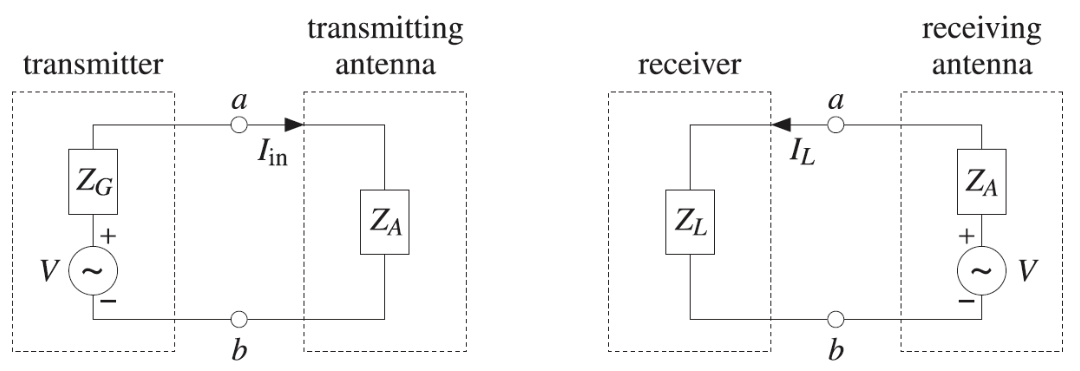
\includegraphics[width = .35\textwidth]{TXRX}
		\end{center}
		
		En RX, $V$ es la tensión en circuito abierto de la antena receptora. $V$ es la tensión en circuito abierto de la antena receptora, depende del campo $E$ o densidad de potencia en la localización de la antena y características de ésa. SI $Z_{A} \neq Z_{L}$ las pérdidas por desadaptación reducen la potencia en $Z_{L}$.
		
		\item \textbf{Impedancia}: Indica si un dispositivo puede ser utilizado como antena o no. La impedancia se puede calcular mediante el coeficiente de reflexión:
			\begin{equation*}
				\rho = \frac{Z_{in} - Z_{o}}{Z_{in} + Z_{o}}
			\end{equation*}
			
		Los analizadores de espectros dan el valor de $Z_{in}$ directamente. Otras medidas relacionadas con $Z_{in}$ y $\rho$ son las \textbf{pérdidas de retorno}:
			\begin{equation*}
				-20 \cdot \log |\rho|
			\end{equation*}
			
		\textbf{COE} (Coeficiente de Onda Estacionaria):
		
			\begin{equation*}
				\text{COE} = \frac{1 + |\rho|}{1 - |\rho|}
			\end{equation*}
		\textbf{Pérdidas por desadaptación}:
		
			\begin{equation*}
				10 \log (1 - |\rho|^{2})
			\end{equation*}
			
		En transmisión, una desadaptación entre el transmisor y la antena puede causar grandes daños en el equipamiento debido a la potencia reflejada.
		
		\item \textbf{Far field radiation region}: A una distancia suficientemente grande de la antena la energía se radia de forma esférica y los frentes de onda pueden ser considerados planos, los campos $\vec{E}$ y $\wedge{H}$ son \textbf{mutuamente perpendiculares}, perpendiculares a la dirección de propagación $\wedge{r}$ y sus módulos están en fase y relacionados con la impedancia intrínseca del medio:

	\begin{equation*}
		\frac{|\vec{E}|}{|\vec{H}|} = \eta
	\end{equation*}
	
La distancia a la cual los campos radiados son considerados como ondas planas y los parámetros de radiación son constantes dependen de la antena y frecuencia. Esta región del espacio se llama far field radiation region. Un valor aproximado para la mínima distancia que asegura la condición far field es:

	\begin{equation*}
		r > \frac{2 D^{2}}{\lambda} \hspace{10pt} \text{D: Largest dimension of the antenna}
	\end{equation*}

	\item \textbf{Densidad de Flujo por Unidad de Área}: O Densidad de potencia obtenida del campo eléctrico y magnético como (rms):
	
		\begin{IEEEeqnarray*}{rCl}
			\vec{W} (\theta, \phi) = \vec{S} (\theta, \phi) & = &  Re \left( \vec{E} x \vec{H} \right) W/m^{2} \\
							   \vec{S} (\theta, \phi) & = & \frac{1}{\eta} \left[ \left| \vec{E}_{\theta} (\theta, \phi) \right|^{2} + \left| \vec{E}_{\phi} (\theta, \phi) \right|^{2} \right]	 \hat{r}
		\end{IEEEeqnarray*}

		Este vector es el valor RMS del vector Poynting. La potencia radiada puede ser calculada como la integral del flujo de potencia a través de una superficie que engloba a la antena:
		
		\begin{equation*}
			P_{r} = \iint_{S} \vec{S} (\theta, \phi) \cdot \partial \vec{s} = \int_{0}^{2\pi} \int_{\theta = 0}^{\theta = \pi} \vec{S} (\theta, \phi) \hat{r} \cdot sin^{2} \cdot  \theta \partial \theta \cdot \partial \phi
		\end{equation*}
	
		\item \textbf{Patrón de Radiación o Patrón de Antena}: Gráfico tridimensional de una de las siguientes magnitudes.

			\begin{IEEEeqnarray*}{rCl}
				\text{Intensidad de Campo Eléctrico Normalizada}&:& 20 \cdot \frac{\left| \vec{E} (\theta, \varphi) \right|}{|\vec{E}_{\text{max}} |} \\
				\text{Densidad de Potencia Radiada Normalizada}&:& 10 \cdot \log \frac{S_{rad} (\theta, \varphi)}{S_{rad_{max}}}
			\end{IEEEeqnarray*}

		Debido a las propiedades de las ondas planas ambos diagramas son iguales y el campo magnético puede ser usado con el mismo resultado. El patrón de radiación es un gráfico que ayuda a visualizar dónde transmite/recibe potencia la antena.\\
		
		En muchos casos es mucho más sencillo y suficiente representar el patrón de radiación mediante cortes. Los más utilizados son $\theta$ constante (paralelo) y $\phi$ constante (meridianos). Para la mayoría de antenas (antenas polarizadas linealmente) hay dos planos principales:
		
			\begin{itemize}
			\item \textbf{Plano E}: Definido por la dirección de la radiación máxima y el vector campo eléctrico en esa dirección.
			\item \textbf{Plano H}: Definido por la dirección de la radiadión máxima y el vector campo magnético en esa dirección.
			\end{itemize}
			
		Los dos planos son perpendiculares y su intersección es la dirección de máxima ganancia. Una onda está polarizada según su plano $\vec{E}$. Si la antena no está polarizada correctamente hay pérdidas de despolarización. Los cortes pueden representarse en coordenadas cartesianas o polares.\\
		
		Las antenas pueden ser clasificadas según su patrón de radiación como:
		
			\begin{itemize}
				\item Antena Isotrópica: Antena ideal que radia de igual forma en todas direcciones. Su patrón de radiación es una esfera.
				\item Antena Omnidireccional: Antena cuyo patrón de radiación tiene una simetría de revolución en un eje. Para definir el diagrama es suficiente dibujar un único corte conteniendo a ese eje.
				\item Antena direccional: El resto de las antenas, una antena que no es isotrópica u omnidireccional.
			\end{itemize}
			
		De los patrones de radiación se suelen diferenciar los siguientes parámetros:
		
			\begin{itemize}
			\item Lobe: Porción de diagrama limitada por las regiones de menor radiación.
			\item Main lobe: El lobe que contiene la máxima dirección de radiación.
			\item Sidelobes: No main lobe.
			\item Lateral lobes: Lobes adyacentes al main lobe
			\item Back lobe: Opuesto a la dirección de máxima radiación
			\item Sidelobe Leven (SSL): The highest side lobe level relative to the main lobe level.
			\item Half Power Beamwidth (HPBW) o 3dB Beamwidth: Ángulo entre half-power points. Da una indicación de la directividad.
			\item Null to Null Beamwidth: \textasciitilde 2,25 HPBW
			\item Front to back: Ratio entre el main lobe y el back lobe.
			\end{itemize}
			
		\item \textbf{Ganancia Directiva}: Definida como el ratio entre la densidad de potencia radiada en una dirección y la densidad de potencia que una antena isotrópica radiaría bajo las mismas condiciones (misma distancia y potencia total radiada).
		
		\item \textbf{Directividad} es la ganancia directiva en la dirección de máxima radiación. Muchas veces la directividad se utiliza para referirse a la ganancia directiva.
		
		\begin{equation*}
			D(\theta, \phi) = \frac{S(\theta, \phi)}{S(\theta, \phi) |_{\text{iso}}} = \frac{S(\theta, \phi)}{\frac{P_{r}}{4 \pi r^{2}}} \hspace{15pt} D = \frac{S_{max}}{\frac{P_{r}}{4 \pi r^{2}}}
		\end{equation*}
		
		\begin{figure}[h]
		\centering
	    	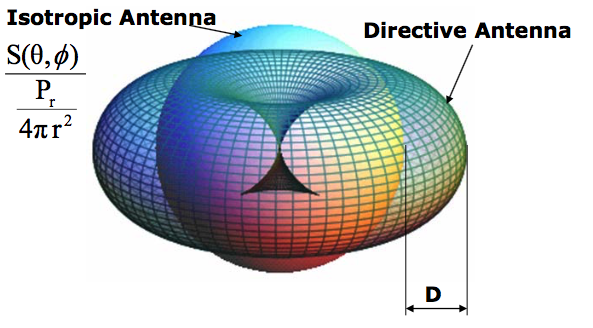
\includegraphics[width = 0.35\textwidth]{images/Directiva}
		\caption{Directividad antena isotrópica y directiva}
		\end{figure}
		
		\item \textbf{Ganancia de una Antena}: Definida de una manera similar a la directividad, en este caso en lugar de compararlo con una antena isotrópica radiando la misma potencia, la comparación se realiza con la densidad de potencia de la antena isotrópica at which se entrega la misma potencia. Como la potencia entregada es mayor que la radiada (debido a las pérdidas), la ganancia es ligeramente menos a la directividad.
		
		\begin{equation*}
		G = \frac{S_{max}}{S_{iso sin perdidas}} = \frac{S_{max}}{\frac{P_{in}}{4 \pi r^{2}}} \hspace{15pt} P_{r} = P_{in} \eta_{l} \hspace{5pt} \rightarrow \hspace{5pt} G = D \eta_{l}
		\end{equation*}
		
		En muchos casos las pérdidas son pequeñas entonces la ganancia y directividad son cuasi idénticas. Ambas, ganancia y directividad, son expresadas en $dB$, si son referidas a la antena isotrópica son $dBi$. Algunas veces, la ganancia o directividad es comparada al dipolo $\lambda / 2$ y es expresado en $dBd$. La directividad del dipolo de $\lambda / 2$ es $1,64$ o $2,15 dBi$, entonces $dBi = dBd + 2,15$. Siempre utilizaremos $dBi$ pero en algunos casos se utilizarán los $dB$.
		
		\item \textbf{PIRE} (\textit{Potencia Isotrópica Radiada Efectiva}): Potencia que tendría que radiar una antena isotrópica para obtener la misma densidad de potencia que produciría una antena direccional en la dirección de máxima radiación. El efecto de la direccionalidad es que en algunas direcciones hay una ganancia de potencia relativa al radiador isotrópico. Se calcula como el producto de la potencia radiada por la directividad.
		
		\begin{equation*}
		D(\theta, \phi) = \frac{S(\theta, \phi)}{\frac{P_{r}}{4 \pi r^{2}}} \rightarrow S(\theta, \pi) = \frac{D(\theta, \phi) \cdot P_{r}}{4 \pi r^{2}} = \frac{\text{PIRE}(\theta, \phi)}{4 \pi r^2} 
		\end{equation*}
		
		\begin{equation*}
		G(\theta, \phi) = \frac{S(\theta, \phi)}{\frac{P_{r}}{4 \pi r^{2}}} \rightarrow S(\theta, \pi) = \frac{G(\theta, \phi) \cdot P_{in}}{4 \pi r^{2}} = \frac{\text{PIRE}(\theta, \phi)}{4 \pi r^2} 
		\end{equation*}
		
		\begin{IEEEeqnarray*}{rCl}
			\textbf{PIRE} & = & D \cdot P_{r} \\
					     & = & G \cdot P_{in}
		\end{IEEEeqnarray*}
	
		\item \textbf{PRA} (\textit{Potencia Radiada Aparente}) es la potencia que tendría que radiar una antena dipolo de media onda para obtener la misma densidad de potencia que produciría una antena direccional en la dirección de máxima radiación. Es la misma definición que PIRE pero utilizando un dipolo de media onda en lugar de una antena isotrópica.
		
			\begin{equation*}
				\text{PIRE} = \text{PRA} + 2.15 (\text{dB})
			\end{equation*}
			
		\item \textbf{Polarización}: Campos electromagnéticos radiados por la antena son vectores y por tanto, su módulo y dirección tienen que ser definidos. Polarización es el parámetro que nos permite determinar la dirección de los campos $E$ y $H$, o al menos cómo varían con en la dirección de propagación o con el tiempo. Realmente, sólo la dirección de uno de los vectores (el campo $E$) tiene que ser definida ya que la otra (campo $H$)j es definida como es una onda electromagnética plana. En general, si se observa cómo varía el vector de campo eléctrico varía con el tiempo desde un punto de vista fijo se observa que describe una elipse. La polarización de una antena es la polarización de las ondas que radia. Normalmente, las antenas se diseñan para tener una polarización linear o circular.  Tanto el transmisor como el receptor tienen que tener la misma polarización o habrá pérdidas.
		
		\item \textbf{Área Efectiva o Apertura}:  Area que cuando es interceptada por la densidad de potencia incidente ($S$) da la cantidad de potencia recibida ($P_{L}$):
		
			\begin{equation*}
			P_{L} = S \cdot A_{ef} \hspace{5pt} \rightarrow \hspace{5pt} A_{ef} = \frac{P_{L}}{S}
			\end{equation*}
			
			El área efectiva no es igual al área física de la antena, está realacionado con la directividad:
			
				\begin{equation*}
				A_{ef} = \frac{\lambda^{2}}{4 \pi} \cdot D
				\end{equation*}
				
		\item \textbf{Factora de Antena o Factor K}: En algunos casos es interesante obtener el valor del campo incidente $E$ del nivel de tensión recibido. Medido en voltios en la carga (típicamente $50 \Omega$).
		
			\begin{equation*}
			|E| = V_{L} \cdot K \hspace{5pt} \rightarrow \hspace{5pt} AF = K = \frac{|E|}{V_{L}}
			\end{equation*}
			
			\begin{equation*}
			K(dB) = 20 \cdot \log \frac{|E|}{V_{L}} dBm^{-1}
			\end{equation*}
			
			Si la antena está adaptada a la carga:
			
			\begin{equation*}
			P_{L} = \frac{V_{L}^{2}}{R_{r}} = \frac{|E|^{2}}{\eta} A_{ef} \hspace{5pt} \rightarrow \hspace{5pt} K = \left( \frac{\eta}{R_{r}} \cdot \frac{1}{A_{ef}} \right)^{\frac{1}{2}}
			\end{equation*}
			
			Para $R_{r} = 50 \Omega$:
			
				\begin{equation*}
				K = \frac{9,73}{\lambda \sqrt{D}}
				\end{equation*}
		
	\end{itemize}

\subsection{Espacio Libre}

Hasta ahora se ha visto a la antena desde un punto de vista de transmisión o recepción, ahora se estudiará el punto de vista del sistema transmisor-receptor en espacio libre. Para diseñar un sistema de radio es necesario hacer un balance de potencia en el que el receptor tenga suficiente potencia para alcanzar el mínimo calor de $C/N$ para la correcta recepción. La densidad de potencia radiada por una antena isotrópica es:

	\begin{equation*}
	S = \frac{P_{\text{radiada}}}{4 \pi r^{2}}
	\end{equation*}
	
Las antenas reales presentan un comportamiento directivo, en este caso la densidad de potencia es obtenida como en la antena isotrópica pero usando PIRE:

	\begin{equation*}
	S =  \frac{D \cdot P_{\text{radiada}}}{4 \pi r^{2}} = \frac{G \cdot P_{in}}{4 \pi r^{2}} = \frac{\text{PIRE}}{4 \pi r^{2}}
	\end{equation*}

La antena de recepción transferirá parte de la densidad de potencia a potencia en la carga:

	\begin{equation*}
	P_{L} = S \cdot A_{ef} = \frac{P_{rad}}{4 \pi r^{2}} \cdot D_{T} A_{ef_{R}} = \frac{P_{rad}}{4 \pi r^{2}} \cdot D_{T} D_{R} \frac{\lambda^{2}}{4 \pi}
	\end{equation*}
	
	\begin{equation*}
	\frac{P_{L}}{P_{rad}} = \left( \frac{\lambda}{4 \pi r} \right)^{2} D_{T} D_{R}
	\end{equation*}
	
	\begin{equation*}
	\frac{P_{RX}}{P_{in}} = \left( \frac{\lambda}{4 \pi r} \right)^{2} G_{T} G_{R}
	\end{equation*}

\textbf{Pérdidas del Espacio Libre}

	\begin{equation*}
	L_{0} = L_{FSL} = \left( \frac{4 \pi r}{\lambda} \right)^{2} \hspace{20pt} L_{FSL} (dB) = 20 \cdot \log \left( \frac{4 \pi r}{\lambda} \right)
	\end{equation*}

\begin{equation*}
P_{RX} - P_{rad} = -L_{FS_{L}} + D_{T} + D_{R} - L \hspace{15pt} (dB)
\end{equation*}

El término $L$ tiene en cuenta otras pérdidas (óhmicas en la antena de transmisión, gas, atenuación por lluvia...). Utilizando antenas isotrópicas $L_{FSL}$ y una separación entre TX y RX $\lambda$ metros la atenuación es aproximadamente $22dB$.

\subsection{Link Budget}

Link Budget es el recuento de todas las ganancias y pérdidas del transmisor a través del medio hasta el receptor. Cuenta la atenuación de la señal transmitida debido a la propagación, como también la ganancia de la antena, feedline y otro tipo de pérdidas. También se tiene en cuenta, añadiendo un margen, ganancias aleatorias que varían. El objetivo del link budget es asegurarse de que el nivel de señal es suficientemente alto como para llegar al receptor.

\begin{figure}[h]
	\centering
     \begin{tikzpicture}
     
%	   \draw [red,thick,domain=250:110] plot ({cos(\x)}, {sin(\x)});
	   \draw (1,1)[red,thick,domain=290:70] plot ({cos(\x)}, {sin(\x)});
% 	\node at (0,0) [circle,draw] (Antena1) {Antena};
        \node at (3,0) [rectangle,draw] (Transmisor) {Transmisor};
        \node at (6,0) [rectangle, draw] (Linea) {Linea de TX};
        \draw (8,-1) arc (250:110:1);
%        \node at (0,-2) [rectangle, draw] (Transmisor){Transmisor};
%        \node at (3,-2) [rectangle,draw] (Perturbaciones){Perturbaciones};
%        \node at (6,-2) [rectangle, draw] (Receptor){Receptor};
%        \node at (0,-4) [circle,draw](Fuente)  {Fuente};
%        \node at (6,-4) [circle,draw](Display) {InfoDisplay};
%        
%        
        \draw[->, blue, thick] (Transmisor) -- (Linea);
        \draw[->, blue, thick] (Linea) -- (7.5,0);
%        \draw[->, red, thick] (Antena1) -- (Medio);
%        \draw[->, red, thick] (Medio) -- (Antena2);
%        \draw[->, blue, thick] (Receptor) -- (Display);
%        \draw[->, blue, thick] (Perturbaciones) -- (Receptor);
%        \draw[->, blue, thick] (Perturbaciones) -- (Transmisor);
%        \draw[->, blue, thick] (Perturbaciones) -- (Medio);
%        \draw[->, blue, thick] (Antena2) -- (Receptor);
%        
%	\node at (3,-4) [blue] {Señal};
%	\node at (3,-4.3) [red]{Radiación};

	\end{tikzpicture}
      \caption{Esquema general}
  \end{figure}
  
  \textbf{TERMINAR LO DE ARRIBA}

	\begin{IEEEeqnarray*}{rCl}
		P_{L} - P_{rad} & = & - L_{FSL} + D_{T} + D_{R} - L \\
		P_{RX} - P_{in} & = & -L_{FSL} + G_{T} + G_{R} - L
	\end{IEEEeqnarray*}
	
$L$ no incluye las pérdidas óhmicas.

\hrulefill

\subsection{Ruido e Interferencias}

El \textbf{ruido de radio} es definido por la ITU-R como un fenómeno electromagnético dependiente del tiempo que tiene componentes en el rango de la radiofrecuencias. El ruido está presente en todos los equipos de comunicación. Fuentes de ruido:

	\begin{itemize}
	\item \textbf{Ruido externo}: La antena de recepción recibe señales indeseadas.
	\item \text{Ruido interno}: Los componentes de la cadena de recepción añaden ruido.
	\end{itemize}
	
Normalmente, el ruido es AWGN:
	
	\begin{itemize}
	\item \textbf{Aditivo}: La potencia de diferentes fuentes de ruido es añadida directamente.
	\item \textbf{Blanco}: La densidad espectral de potencia es plana en la banda de frecuencias de interés.
	\item \textbf{Gaussiano}: Su valor instantáneo es una variable aleatoria que sigue una distribución gaussiana con media cero y varianza $\sigma^{2}$.
	\end{itemize}

La temperatura de ruido de una antena es utilizada para calcular la potenciad e ruido recibida por la antena:

	\begin{equation*}
	N = k T_{a} B
	\end{equation*}

Este ruido es atenuado por las pérdidas de la antena:

	\begin{equation*}
	N = kT_{a} B \eta_{l}
	\end{equation*}
	
El ruido debido a la antena produce el mismo efecto que un atenuador:

	\begin{equation*}
	\text{Atenuador: } T_{e} = T_{\text{amb}} (l - 1) \hspace{5pt} \rightarrow \hspace{5pt} N = k T_{\text{amb}} B (1 - \eta_{l})
	\end{equation*}

La potencia total de ruido a la salida es:

	\begin{equation*}
	N = k T_{a} B \eta_{l} + k T_{\text{amb}} B (1 - \eta_{l})
	\end{equation*}
	
\subsubsection{Ruido en la cadena de recepción}

Cada elemento en la cadena tiene dos efectos en el ruido, atenuar o amplificar el ruido proveniente de etapas anteriores (ganancias o pérdidas). Añade algo de ruido internamente generado por el elemento. El ruido añadido por cualquier elemento puede ser cuantificado por cualquiera de los siguientes parámetros:

	\begin{itemize}
	\item Temperatura de ruido equivalente ($T_{e}$) es la temperatura de una resistencia puesta en la entrada que genera la misma potencia de ruido  a la salida que el elemento. Si se conoce $T_{e}$, el ancho de banda y la ganancia, también se puede conocer la potencia de ruido a la salida. De un elemento pasivo $T_{e} = T_{\text{amb}} (l -1)$.
	\item Factor de ruido o figura ($f$ o $F$) es el ratio de $S/N$ a la entrada y a la salida de un elemento cuando la potencia de ruido a la entrada es $N = k T_{0} B$. Es una medida de calidad del elemento, es mejor cuanto más cercano a 1 es. Normalmente dado en $dB$ como $F = 10 \cdot \log f$. Es otra forma de cuantificar el ruido interno, $T_{e}$ puede ser calculado como factor de ruido
	
		\begin{equation*}
		f = \frac{(S/N)_{i}}{(S/N)_{o}} = \frac{\frac{S}{k T_{0} B}}{\frac{S \cdot g}{k (T_{0} + T_{e}) g B}} = \frac{T_{0} + T_{e}}{T_{0}} \hspace{5pt} \rightarrow \hspace{5pt} T_{e} = f \cdot T_{0} - T_{0} 
		\end{equation*}
		
		\begin{equation*}
		T_{e} = T_{0} (f - 1) \hspace{10pt} \text{Si} f \gg 1 \rightarrow T_{e} \approx T_{0} f
		\end{equation*}
		
		Cuando  la temperatura ambiente es la de referencia, el fator de ruido de un atenuador es igual a su atenuación.
		
		\begin{equation*}
		T_{e} = T_{\text{amb}} (l - 1) \hspace{5pt} \text{si} T_{\text{amb}} = T_{0} \hspace{5pt} \rightarrow \hspace{5pt} T_{e} = T_{0} (l - 1) \hspace{5pt} \rightarrow \hspace{5pt} f = l
		\end{equation*}
		
	\item Potencia de ruido: $N$
	\end{itemize}
	
La \textbf{interferencia} se define por la ITU como el efecto de energía indeseada debido a una o una combinación de emisiones, radiaciones o inducciones en la recepción en un sistema de radiocomunicaciones manifestado por cualquier degradación en el rendimiento o pérdida de información que podría haber sido extraída en ausencia de dicha energía indeseada. En muchos aspectos es similar al ruido, debido a que ambos producen una degradación de potencia en el receptor, pero el ruido es incorrelado a la señal mientras que en el caso de la interferencia no es siempre cierto. 

\subsection{Medidas de Calidad}

En transmisiones analógicas $S/N$ o $SNR$. En transmisiones digitales, relacionado con las modulaciones está el \textbf{MER} y el EVM. Un error es un vector en el plano IQ entre el punto ideal de la constelación y el punto recibido por el receptor.\\

\textbf{Probabilidad de error}, asumiendo codificación Gray, es:

	\begin{equation*}
	P_{eb} = k \cdot G (d / \sigma)
	\end{equation*}
	
Donde $D$ es la distancia de decisión en los puntos de constelación. $k$ es una constante que depende del tipo de modulación. $\sigma$ es un aditivo normalizado de la potencia de ruido Gaussiano blanco en el receptor. $G(t)$ es la función de distribución complementaria Gaussiana.\\

El ratio $d / \sigma$ puede ser normalizado en términos de energía de bit a ratio de desnidad de ruido $e_{b} / n_{o}$. En los esquemas de modulación con amplitudes envelope variables, la energía por bit será expresada según al máxima amplitud de la portadora modulada, $A$.

	\begin{equation*}
	\frac{c}{n} = \frac{e_{b}}{n_{0}} \cdot \frac{T_{s}}{T_{b}} = \frac{e_{b}}{n_{0}} \cdot \log_{2} M
	\end{equation*}
	
	
\hrulefill

\section{\underline{3. Propagación}}





















\hrulefill


\newpage

Falta dónde poner esto:

\begin{figure}[h]
	\centering
     \begin{circuitikz}[scale=.8, transform shape, european]

	\draw[fill] (-.15,0) circle[radius = 1pt];
	\draw[fill] (-.15,-2) circle[radius = 1pt] node[below]{g};
	\draw[fill] (5, -2) node[below]{d};
	
	\draw (-3,0) 
		to[sV, l_= $V_{TX}$] (-3,-2)
		(-3,0) to[R  = $Z_{O}$] (0,0);
	\draw (0,0) 
		to[R  = $R_{\Omega}$] (2,0)
		to[R  = $jX_{in}$] (4,0)
		-- (5,0)
		to[R  = $R_{r}$] (5,-2)
		-- (-3,-2);
		
	\draw[-latex] (-.3,-1.9) -- (-.3,-.1) node[midway, left] {$P_{in}^{'}$};
	\draw[-latex] (0,-1.9) -- (0,-.1) node[midway, right] {$P_{in}$};
	
	\draw (-1.5, -.5) node[]{(1)};
	\draw (2.5, -.5) node[left]{(2)};
\end{circuitikz}
      \caption{Antena Transmisora}
  \end{figure}
	
Las \textbf{pérdidas por desadaptación} (1) se producen en el generador del transmisor y las \textbf{pérdidas de desadaptación} en la antena transmisora.

	\begin{IEEEeqnarray*}{rCl}
		Z_{in} & = & R_{in} \\
		X_{in} & = & R_{R} + R_{\Omega} + j \cdot X_{in}
	\end{IEEEeqnarray*}

La potencia 

	\begin{IEEEeqnarray*}{rCl}
		P_{in} & = & P_{in}^{'} (1 - |\rho|^{2}) \\
		P_{R} & = & \eta \cdot P_{in} = I^{2} \cdot R_{R}
	\end{IEEEeqnarray*}	
	
Donde:

	\begin{equation*}
	\rho = \frac{Z_{in} - Z_{O}}{Z_{in} + Z_{O}} \hspace{20pt} \eta = \frac{R_{R}}{R_{R} + R_{\Omega}}
	\end{equation*}
	
En el aire se trabaja con densidad de potencia:

	\begin{equation*}
	D \text{y} S \rightarrow S = \frac{P_{r}}{4 \pi r^2} \cdot D = \frac{P_{in}}{4 \pi r^{2}} \cdot G = \left( \frac{W}{m^{2}} \right)
	\end{equation*}

	\begin{IEEEeqnarray*}{rCl}
		S & = & E \cdot H \\
		\left( \frac{W}{m^{2}} \right) & = & \left( \frac{V}{m} \right) \cdot \left( \frac{A}{m} \right)
	\end{IEEEeqnarray*}	
	
	\begin{equation*}
		G \cdot P_{in} = D \cdot P_{r}	
	\end{equation*}
	
Onda plana (campo lejano): $E = H \cdot \eta_{0}$ con $\eta_{0} = 120 \pi (\Omega)$.\\

\textbf{Antena Receptora}: La energía la da la antena receptora, no es un generador pero actúa como él.

\begin{figure}[h]
	\centering
     \begin{circuitikz}[scale=.8, transform shape, european]

	\draw[fill] (4,0) circle[radius = 1pt];
	\draw[fill] (4,-2) circle[radius = 1pt] node[below]{$g_{RX}$};
	\draw[fill] (-2, -2) circle[radius = 1pt] node[below]{$d_{RX}$};
	
	\draw (-3,0) 
		to[sV, l_= $V_{TX}$] (-3,-2)
		(-3.5,-1) node[right]{$P_{RX}$}
		(-3,0) to[R  = $R_{r}$] (0,0);
	\draw (0,0) 
		to[R  = $R_{\Omega}$] (2,0)
		to[R  = $jX_{in}$] (4,0)
		-- (5.5,0)
		to[R  = $R_{RX}$] (5.5,-2)
		-- (-3,-2);
		
	\draw[-latex] (3.9,-1.9) -- (3.9,-.1) node[midway, left] {$P_{RX}^{'}$};
	\draw[-latex] (3.9,-1.9) -- (3.9,-.1) node[midway, right] {$P_{RX}$};
	\draw[-latex] (0,-1.9) -- (0,-.1) node[midway, left] {$P_{L}$};
	
	\draw[dashed] node[draw,minimum width=2cm,minimum height=2.4cm,anchor=south west] at (4.9,-2.2){}
		(6,-2.4) node[]{Bloque Receptor};
		
	\draw (-.4, -.5) node[]{(1)};
	\draw (6.5, -.5) node[left]{(2)};
\end{circuitikz}
      \caption{Antena Receptora}
  \end{figure}
 
 Las \textbf{pérdidas óhmicas} (1) se producen en el generador y las \textbf{pérdidas por desadaptación} (2) se producen en el bloque receptor.\\
  
$P_{L}$ es la potencia generada de la antena, no tiene en cuenta las pérdidas óhmicas. Se reciben $\left( \frac{W}{m^{2}} \right)$, para pasarlo a $W$ multiplicar $S$ por el área efectiva de la antena:

	\begin{equation*}
	S \cdot A_{ef} = \left( \frac{W}{m^{2}} \right) \cdot m^{2} 
	\end{equation*}
	
Donde:

	\begin{equation*}
	A_{ef} = \frac{\lambda^{2}}{4 \pi} \cdot D_{RX} (m^{2})
	\end{equation*}

\textbf{?`Qué potencia llega a $R_{RX}$?}:

	\begin{IEEEeqnarray*}{rCl}
		\text{P.Ohmicas}&:& P_{RX}^{'} = P_{L} \cdot \eta_{l_{RX}} \hspace{10pt} \eta_{l_{RX}} = \frac{R_{r}}{R_{r} + R_{\Omega}} \\
		\text{P.Desadaptacion}&:& P_{RX} = P_{RX}^{'} (1 - |P_{RX}|^{2}) \hspace{10pt} \rho_{RX} = \frac{Z_{RX} - Z_{ANT_{RX}}}{Z_{RX} + Z_{ANT_{RX}}}
	\end{IEEEeqnarray*}	

	\begin{IEEEeqnarray*}{rCl}
		p_{L} & = & \frac{P_{R} \cdot D_{TX}}{4 \pi r^2} \cdot \frac{\lambda^{2}}{4 \pi} \cdot D_{RX} \\
		          & = & P_{R} \cdot D_{TX} \left( \frac{\lambda}{4 \pi r} \right)^{2} \cdot D_{RX} \\
		P_{L} & = & 10 \cdot \log \left(  P_{R} \cdot D_{TX} \left( \frac{\lambda}{4 \pi r} \right)^{2} \cdot D_{RX} \right) = 10 \cdot \log p_{L}
	\end{IEEEeqnarray*}	
	
	\begin{IEEEeqnarray*}{rCl}
		P_{L} & = & 10 \cdot \log \left(  P_{R} \cdot D_{TX} \left( \frac{\lambda}{4 \pi r} \right)^{2} \cdot D_{RX} \right) = 10 \cdot \log p_{L} \\
		          & = & 10 \cdot \log P_{r} + 10 \cdot \log D_{TX} + 20 \cdot \log \frac{\lambda}{4 \pi r} + 10 \cdot \log D_{RX} \\
		          & = & P_{R} (dB) + D_{TX} (dB) - 20 \log \frac{4 \pi r}{\lambda} + D_{RX} (dB)\\
		          & = & P_{R} (dB) + D_{TX} (dB) + L_{FS} + D_{RX} (dB) \hspace{5pt} \text{\footnote{Ecuación de Propagación en el Espacio Libre de FRIIS}}\\
		          & = & P_{in} (dB) + G_{TX} (dB) + L_{FS} + D_{RX} (dB)
	\end{IEEEeqnarray*}	
	
Donde $ - 20 \log \frac{4 \pi r}{\lambda}$ son las \textbf{LFS} pérdidas de espacio libre.\\

Si se coge $P_{RX}^{'}$ en lugar de $P_{L}$:

	\begin{IEEEeqnarray*}{rCl}
		P_{RX}^{'} & = & P_{in} + G_{TX} - L_{FS} + G_{RX} \\
				 & = & P_{r} + G_{TX} - L_{FS} + D_{RX} 
	\end{IEEEeqnarray*}	

	\begin{equation*}
		P_{r} + D_{TX} - L_{FS} = P_{L} D_{RX}
	\end{equation*}
	
?`Por qué $D_{RX}$ es de signo negativo en la expresión de arriba al despejar?. Al estar trabajando en unidades logarítmicas, una resta en lineal sería una división por lo que $p_{L} / d_{RX}$. Una antena transmisora se le entrega $P_{TX}$ y la concentra $x \cdot d_{TX}$, una antena receptora recibe $P_{RX}$ y la desconcentra $ x / d_{RX} $ de ahí el signo negativo de la expresión.\\

\textbf{?`Por qué $L_{FS}$ es de signo negativo?}

	\begin{equation*}
	L_{FS} = -20 \cdot \log \frac{4 \pi r}{\lambda}
	\end{equation*}

$\frac{4 \pi r}{\lambda}$ siempre será mayor que uno (condición de campo lejano) por lo que el logaritmo dará valores positivos y el resultado con el menos será negativo.\\

\textbf{Unidades de $D_{TX}$}:

	\begin{equation*}
		D_{TX} = \frac{S_{max}}{S_{iso}} = \frac{\frac{W}{m^{2}}}{\frac{W}{m^{2}}} = \text{adimensional}
	\end{equation*}

Según la referencia que se tome las unidades de $D$ son unas u otras:

	\begin{itemize}
	\item Referencia antena isotrópica: $dBi$
	\item Referencia dipolo: $dBd$.
	\end{itemize}

%\vfill




%\end{multicols}

\end{document}